%%%%%%%%%%%%%%%%%%%%%%%%%%%%%%%%%%%%%%%%%%%%%%%%%%%%%%%%%%%%%%%%%
% Tese de Doutorado / Dept. Fisica, CFM, UFSC                   %
% Lacerda@CórregoGrande - Jan/2018                              %
%%%%%%%%%%%%%%%%%%%%%%%%%%%%%%%%%%%%%%%%%%%%%%%%%%%%%%%%%%%%%%%%%

%:::::::::::::::::::::::::::::::::::::::::::::::::::::::::::::::%
%                                                               %
%                          Capítulo 4                           %
%                                                               %
%:::::::::::::::::::::::::::::::::::::::::::::::::::::::::::::::%

%***************************************************************%
%                                                               %
%                        DIG discussion                         %
%                                                               %
%***************************************************************%

\chapter{Discussão}
\label{sec:DIGdisc}
Nosso método de classificação é inspirado em argumentos teóricos e empíricos possui diversos propósitos. Neste capítulo vamos aplicar nosso méotodo para nossa amostra do CALIFA cobrindo alguns objetivos específicos:
\begin{enumerate*}[label=(\roman*)]
    \item estimar a relevância do hDIG, mDIG e SFc sobre galáxias cobrindo toda a sequência de Hubble;
    \item estudar a natureza da emissão difusa extraplanar nos sistemas {\em edge-on};
    \item comparar resultados obtidos com o nosso método frente aqueles que separam SF/DIG baseados em um limite fixo em $\Sigma_{\Ha}$;
    \item investigar a possibilidade de discernimento entre regimes DIG e SF baseados em razões de linhas sensíveis à densidade do meio;
    \item testar a consistência de nosso sistema de classificação analisando através de um diagrama clássico de linhas de emissão;
    \item examinar a mistura presente no mDIG;
    \item fechamos a discussão com os possíveis adversidades em nosso estudo.
\end{enumerate*}

\section{A relevância das componentes hDIG, mDIG e SFc}
\label{sec:DIGdisc:relstrenghts}

%---------------------------- Figure ----------------------------
\begin{figure}
 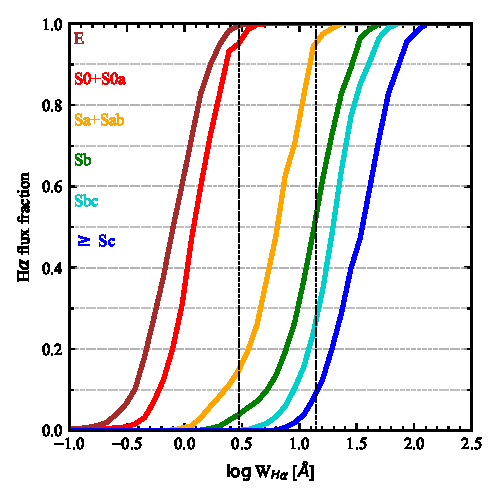
\includegraphics{figuras/fig_cumul_fHaWHa_per_morftype.pdf}
 \caption[Fração cumulativa do fluxo de \Ha com o crescimento de $W_{\Ha}$ para diferentes classes morfológicas]
 {Fração cumulativa do fluxo total de \Ha provenientes de regiões com $W_{\Ha}$ menor que determinado valor. O gráfico mostra as curvas medianas obtidas para galáxias presentes em cada uma de nossas seis classes morfológicas.}
 \label{fig:CurveOfGrowth}
\end{figure}
%---------------------------- Figure ----------------------------

Dentre as questões que podemos perscrutar neste estudo, a importância relativa das componentes de nossa classificação talvez seja a mais importante. A dominância e a evolução da influência que cada um dessas componentes tem sobre galáxias através de diferentes tipos morfológicos é importante na interpretação de propriedades derivadas de dados espectrais não resolvidos espacialmentes. Nesses estudos as assinaturas de regimes distintos vêm todas misturadas sob o mesmo espectro.

Uma maneira simples e relevante observacionalmente de quantificar isso é calculando a contribuição relativa de cada componente para o fluxo total de \Ha. Por exemplo, nas galáxias na Figura \ref{fig:ExampleMaps} essas frações vão de $(f_{\rm hDIG} , f_{\rm mDIG} , f_{\rm SFc}) = (87,13,0)$ para a galáxia S0 CALIFA 0072, até $(5.5,47,47.5)$ para a galáxias Sb CALIFA 0010, e $(0.3,46.1,53.6)$ para a CALIFA 0813, uma Sbc. Essa progressão ao longo da sequência de Hubble reflete as tendências que podem ser vistas na Figure \ref{fig:WHaDistrib_ALLgals}. No canto superior direito de cada painel temos os valores de $(f_{\rm hDIG} , f_{\rm mDIG} , f_{\rm SFc})$ para diferentes distâncias radiais e diferentes tipos morfológicos.

De maneira mais elaborada, a Figura \ref{fig:CurveOfGrowth} mostra essas frações para toda a amostra através dos valores medianos de cada classe morfológica. Nós calculamos a fração cumulativa do fluxo de \Ha, $f$, proveniente de regiões que possuem $W_{\Ha}$ menor que determinado valor. As curvas de $f(<W_{\Ha})$ representam como a fração cumulativa cresce com relação a $W_{\Ha}$. Na figura mostramos as curvas medianas para as nossas seis classes morfológicas. As linhas tracejadas verticais representam nossas fronteiras hDIG/mDIG e mDIG/SFc, em 3 e 14 \AA\ respectivamente.

A progressão constante de {\em early-} para {\em late-types} nessas curvas confirmam nossas expectativas provenientes das distribuições de $W_{\Ha}$ (Figura \ref{fig:WHaDistrib_ALLgals}) além de também nos permitir quantificar a importância relativa entre as componentes e o fluxo total de \Ha. Em galáxias elípticas ou S0 temos praticamente toda a emissão de \Ha na fase hDIG ($W_{\Ha} \le 3$). Entre os sistemas Sa-Sab, essa componente se encarrega por 14\% do fluxo de \Ha, com o mDIG sendo o responsável por praticamente todo o fluxo restante. De Sb para frente, o regime SFc domina, sendo responsável por 50\% ou mais. Natualmente existe um espalhamento natural nos dados, mesmo quando divididos em classes morfológicas.

A contribuição relativa do DIG para a emissão em \Ha foi estimada em diversos estudos anteriores, geralmente baseados em dados obtidos com filtros estreitos (\Ha + \nii) \citep{Ferguson.etal.1996, Zurita.etal.2000, Thilker.etal.2002, Oey.etal.2007}, com resultados variando substancialmente principalmente devido a diferenças na metodologia de separação da emissão difusa. O maior estudo até hoje foi feito por \citet{Oey.etal.2007}, que estimaram a fração de emissão difusa em \Ha de $59\pm19 \%$ sobre uma amostra de 109 galáxias do {\em survey} SINGG \citep{Meurer.etal.2006}. Para nossa amostra (e nossas definições) nós encontramos um valor bem próximo, 56\% (hDIG + mDIG), mas com um espalhamento muito maior, $\pm38 \%$. Diferentemente de nosso estudo (Figura \ref{fig:CurveOfGrowth}), eles não encontraram nenhuma evidencia de correlação com o tipo morfológico. Talvez o motivo seja devido a diferença de critério e metodologia de classificação DIG/SF.


\section{Emissão extraplanar em sistemas {\em edge-on}}
\label{sec:DIGdisc:edgeon}

%---------------------------- Figure ----------------------------
\begin{figure}
 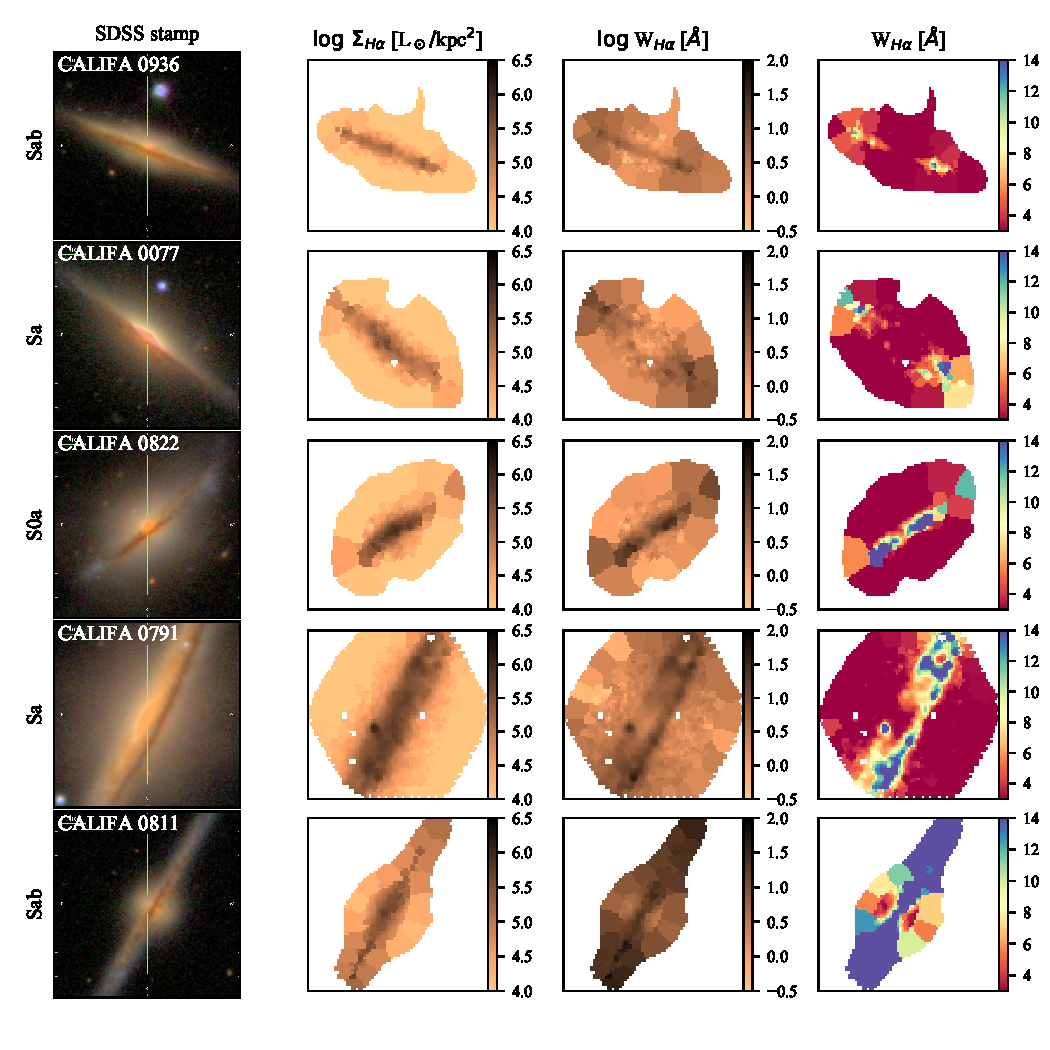
\includegraphics{figuras/fig_maps_class_edgeon_paper.pdf}
 \caption[Imagem \SDSS e mapas de $\Sigma_{H\alpha}$ e $W_{H\alpha}$: sistemas {\em edge-on}]
 {Como a Figura.\ \ref{fig:ExampleMaps}, mas para galáxias {\em edge-on}.}
 \label{fig:ExampleMapsEdgeOn}
\end{figure}
%---------------------------- Figure ----------------------------

Devido ao comportamento sistemático das propriedades de linhas de emissão, esses sistemas altamente inclinados são importantes para o estudo da emissão DIG nas regiões acima (e abaixo) do disco galáctico \citep{Tullmann.and.Dettmar.2000, Otte.etal.2002, Jones.etal.2017}. A galáxia protótipo utilizada nesses estudos é a NGC 891, extensivamente observada em diversos comprimentos de onda \citep{Rand.1998, Hodges.and.Bregman.2013, Seon.etal.2014, Hughes.etal.2015}. Esses estudos enfatizaram que as propriedades de linhas de emissão observadas no DIG extraplanar não podem ser explicadas puramente por fótons Lyman que escapam de regiões \hii presentes no disco. Uma variedade de fenômenos que pudessem gerar tal emissão foram sugeridos, como: dissipação de turbulência \citep{Minter.and.Spangler.1997}, reconexão magnética \citep{Raymond.1992}, choques \citep{Collins.and.Rand.2001}, raios cósmicos, aquecimento fotoelétrico proveniente de grãos de poeira do meio interestelar  \citep{Weingartner.and.Draine.2001}, e fótons Lyman vindos de estrelas velhas e quentes \citep{FloresFajardo.etal.2011a}.

A Figura \ref{fig:ExampleMapsEdgeOn} nos mostra como os dados do CALIFA podem nos trazer um novo {\em insight} ao problema. Nela vemos cinco exemplos de galáxias {\em edge-on} dispostas da mesma forma que na Figura \ref{fig:ExampleMaps}. As quatro primeira possuem configuração muito parecida, onde temos o disco e arredores dominados por mDIG e SFc, enquanto a grandes distâncias do disco galácticos vemos uma completo predomínio de hDIG. Isso favorece o cenário proposto por \citet{FloresFajardo.eteal.2011a}, onde a ionização se torna dominada por HOLMES à medida que nos afastamos do plano galáctico. Essa conclusão é reforçada pelos mapas de diagnóstico de razões de linhas baseados em dados do MaNGA em \citet{Belfiore.etal.2016} e \citet{Zhang.etal.2017a}.

Através de nossa experiência calculando $\xi$ (veja a Seção \ref{sec:DIGclass:WHaDistrib_hDIG})


%% End of this chapter
